\hfill \newline
\phantom{ } Then we built the summing aplifier circuit according to the figure below. We kept the power supply at $ \mathrm{V_s} = \pm12\si{V} $, and set the function generator to provide ${v_1}(t)=cos(2000\pi t)\si{V}$, ${v_2}(t)={v_3}(t)=0$. All resistors wereset to $100\si{k\Omega}$ and the capacitor $C=22\si{pF}$.
\begin{figure}[!htbp]
	\centering 
	\begin{framed}
		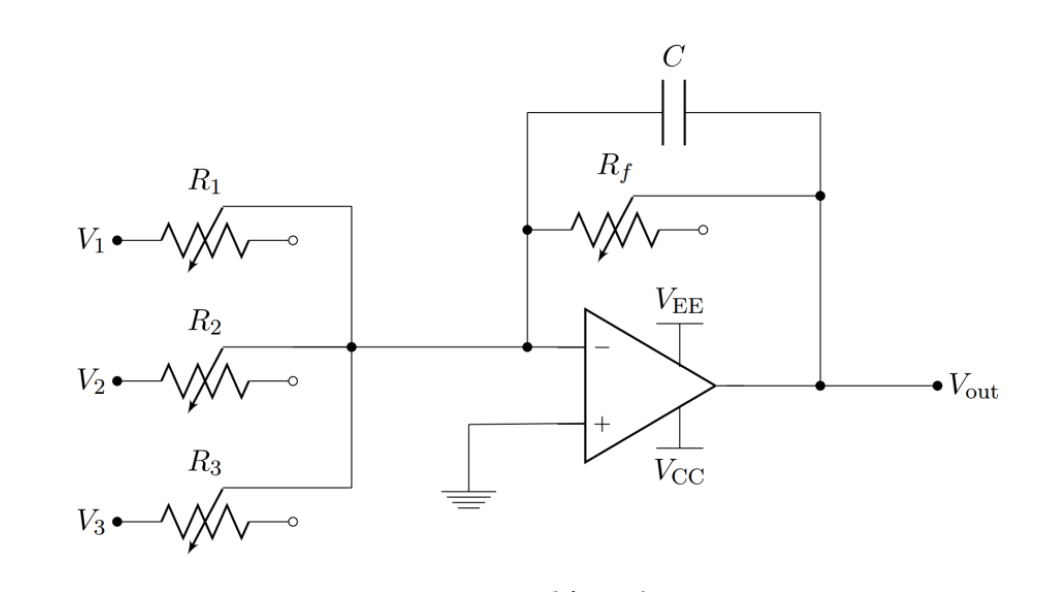
\includegraphics[width=\linewidth]{images/summing_amp.PNG} 
		\caption{Summing amplifier with potentiometers}
		\label{fig:samp} 
	\end{framed}
\end{figure} 

\phantom{ } We swept the frequency of $\mathrm{V_1}$ from 10Hz to 1MHz, kept the input amplitude same and recorded the amplitude of output signals. The data collected is showed in Table[\ref{tab:caf}], and we got a plotted figure Figure[\ref{fig:afreq}] of the output voltage in terms of frequency.

\begin{table}[!htbp]
	\centering
	\caption{Amplitudes under different frequencies}
	\begin{tabular}{lccllcc}
		\toprule
		No&freq(Hz)&Amp(V)&&No&freq(Hz)  &Amp(V)\\
		\midrule
		1	&10		&1.94	&&9 &$5*10^3$&2.02\\
		2	&20		&1.94	&&10&$1*10^4$&2\\
		3	&50		&1.94	&&11&$2*10^4$&1.92\\
		4	&100	&1.94	&&12&$5*10^4$&1.55\\
		5	&200	&1.92	&&13&$1*10^5$&1.05\\
		6	&500	&1.96	&&14&$2*10^5$&0.604\\
		7	&1000	&1.96	&&15&$5*10^5$&0.28\\
		8	&2000	&1.98	&&16&$1*10^6$&0.152\\
		\bottomrule
	\end{tabular}
	\label{tab:caf}
\end{table}

\begin{figure}[!htbp]
	\centering 
	\begin{framed}
		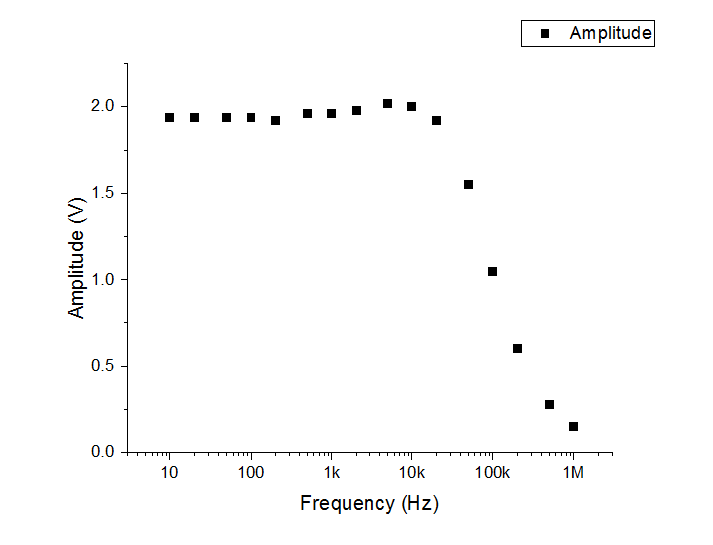
\includegraphics[width=\linewidth]{images/amp_freq.PNG} 
		\caption{Amplitudes under different frequencies}
		\label{fig:afreq} 
	\end{framed}
\end{figure} 

\textbf{Analyze \#4:} \newline
\phantom{ } Comparing our result to Figure[\ref{fig:pre8}], which was plotted in Prelab\#8 and \#11, 
\begin{figure}[!htbp]
	\centering 
	\begin{framed}
		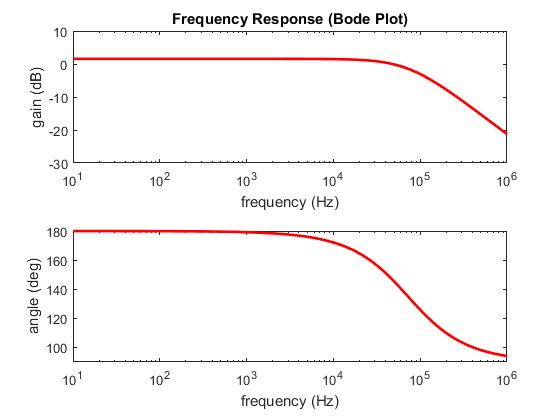
\includegraphics[width=\linewidth]{prelab/images/9_1.PNG} 
		\caption{Magnitude and phase of the output signal}
		\label{fig:pre8} 
	\end{framed}
\end{figure} 